\documentclass[conference]{IEEEtran}
\IEEEoverridecommandlockouts
% The preceding line is only needed to identify funding in the first footnote. If that is unneeded, please comment it out.
\usepackage{cite}
\usepackage{amsmath,amssymb,amsfonts}
\usepackage{algorithmic}
\usepackage{graphicx}
\usepackage{textcomp}
\usepackage{xcolor}
\usepackage{float}
\usepackage{xfp}
\usepackage[section]{placeins}
\begin{document}
	
	\section*{Methodology}
	
	The proposed scheme consists of several sub modules as
	shown in the flow diagram in Fig.\ref{fig:k1}. All the modules of the
	proposed scheme have been written in Python 3.9.
	
	\begin{figure}[H]
		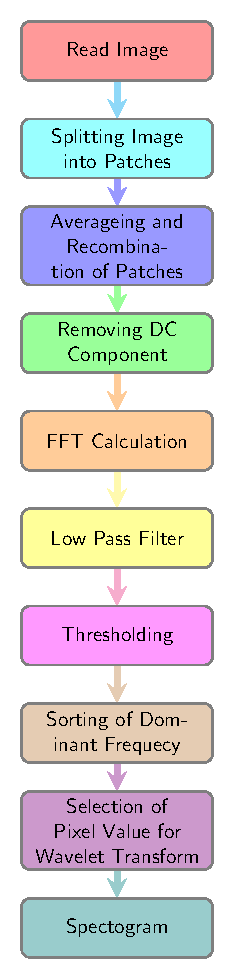
\includegraphics[scale=1.11]{plot/meth.pdf}
		\caption{Flowchart of the image processing procedure}\label{fig:k1}
			\end{figure}
	
\end{document}